\documentclass[12pt]{article}
\usepackage[spanish]{babel}
\usepackage[hyperindex]{hyperref}
\usepackage{graphicx}
\usepackage{enumitem}
\usepackage{verbatim}

\addto\captionsspanish{\renewcommand{\contentsname}{Tabla de Contenidos}}

\begin{document}

\newsavebox\myv % For fixing verbatim input dimensions

\title{\textbf{Modelos y Optimización 1} \\ \large \textbf{Trabajo Práctico 1}}
\author{\begin{tabular}{p{0.3\textwidth}p{0.3\textwidth}p{0.3\textwidth}}
    Bilbao, Manuel & Locatelli, Santiago & Rolando, Marcos \\
    102732 & 104107 & 102323 \\
    \end{tabular}}
\date{9 de abril de 2023}

\maketitle % Prints the title, author, and date

\begin{figure}[htbp]
    \centering
    
\includegraphics[width=0.5\textwidth]{../assets/fiuba.png}
    \label{fig:image}
\end{figure}

\newpage
\thispagestyle{empty}
\tableofcontents
\newpage

\setcounter{page}{1}

\section{Análisis de la situación}

El enunciado nos plantea una situación en la que hay dos tipos
de equipos diferentes, de Combate y Apoyo, cada uno de ellos
compuesto por ciertos elementos en cantidades especificadas.
También nos establece una relación entre los tipos de equipos.
Por cada dos equipos de Combate debe haber \textbf{al menos 
un equipo de Apoyo.}

Por cada equipo armado se obtienen ciertos puntos de mejora.
El equipo de Combate otorga 10 puntos mientras que el equipo
de Apoyo otorga 8 puntos.

En base a lo planteado por el enunciado, lo mejor que puede
hacer el Ministerio es obtener la mayor cantidad de puntos posibles
dada la cantidad de elementos disponibles, por
lo que estamos frente a un problema de \textbf{maximización}.

\section{Objetivo}

Determinar la cantidad de equipos de Combate del Fuego y Apoyo
Logístico a conformar por el Ministerio para maximizar la eficacia
del plan durante la próxima temporada.

\section{Hipótesis y supuestos}

% bullet list
\begin{itemize}
\item Las máquinas y vehículos no se rompen.
\item Los empleados no se ausentan.
\item Los equipos de combate de fuego son indistinguibles entre sí.
\item Los equipos de apoyo logístico son indistinguibles entre sí.
\item Cualquier combinación de equipos aporta los mismos puntos de mejora.
\item No existen causas que hagan que los equipos no tengan la mejora mencionada en el enunciado.
\item Un equipo debe estar completamente integrado por los elementos correspondientes para mejorar la eficacia del plan.
\end{itemize}

\section{Modelo}

\subsection{Variables}

Este problema puede modelarse mediante las siguientes dos variables

\begin{itemize}
\item $C$: Cantidad de equipos de Combate de Fuego a conformar en la temporada. \textbf{[C]}: $\frac{equipos}{temporada}$
\item $A$: Cantidad de equipos de Apoyo Logístico a conformar en la temporada. \textbf{[A]}: $\frac{equipos}{temporada}$
\end{itemize}

\subsection{Funcional}

El funcional planteado para el modelo es el siguiente

$$Max Z = 10\frac{puntos}{equipo} \cdot C + 8\frac{puntos}{equipo} \cdot A$$

\subsection{Restricciones}

A continuación se enumeran las restricciones correspondientes al modelo

\begin{enumerate}[label=(\textbf{\arabic*})]
    \item $2 \cdot A \geq C$
    \item $2 \frac{autobombas}{equipo} \cdot C \leq 16 \frac{autobombas}{temporada}$
    \item $1 \frac{helic\acute{o}pteros}{equipo} \cdot A \leq 8 \frac{helic\acute{o}pteros}{temporada}$
    \item $2 \frac{brigadas}{equipo} \cdot C + 1 \frac{brigadas}{equipo} \cdot A \leq 28 \frac{brigadas}{temporada}$
    \item $1 \frac{drones}{equipo} \cdot C + 2 \frac{drones}{equipo} \cdot A \leq 24 \frac{drones}{temporada}$
\end{enumerate}

\pagebreak
\section{Resolución}

\subsection{Modelo de GLPK}

\verbatiminput{resolucion.mod}

\subsection{Solución obtenida}

\begin{lrbox}{\myv}\begin{minipage}{\textwidth}
\verbatiminput{resolucion.sol}
\end{minipage}\end{lrbox}

\resizebox{0.82\textwidth}{!}{\usebox\myv}

\newpage

\subsection{Solución gráfica}

\begin{figure}[htbp]
    \centering
    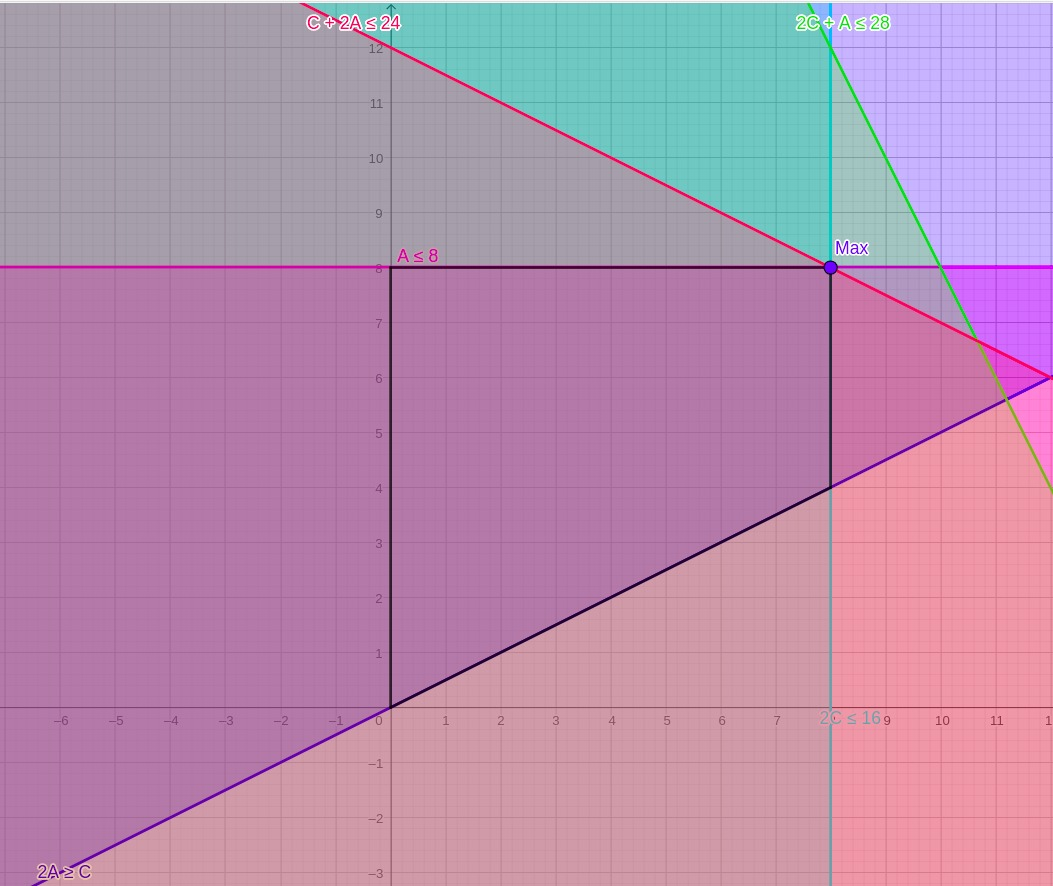
\includegraphics[width=1\textwidth]{../assets/resolucion-grafica.jpeg}
\end{figure}

Se puede observar en la imagen el poliedro formado por las restricciones del modelo,
delineado con el color negro. Se etiquetó como ``Max"\ al vértice del poliedro
que maximiza el funcional, siendo el mismo el punto (8, 8). Podemos notar que este
vértice es un punto degenerado ya que se cruzan tres aristas en el mismo. Las restricciones
correspondientes en este cruce son:

\begin{itemize}
    \item $2 \frac{autobombas}{equipo} \cdot C \leq 16 \frac{autobombas}{temporada}$
    \item $1 \frac{helic\acute{o}pteros}{equipo} \cdot A \leq 8 \frac{helic\acute{o}pteros}{temporada}$
    \item $1 \frac{drones}{equipo} \cdot C + 2 \frac{drones}{equipo} \cdot A \leq 24 \frac{drones}{temporada}$
\end{itemize}

\section{Conclusiones}

En base a lo observado en la solución gráfica podemos extraer como conclusión que si quisiéramos maximizar aún más
la eficacia del plan los elementos que se deberían comprar u obtener son helicópteros, autobombas
y drones en la proporción correspondiente. En otras palabras, si solo se consiguiera más helicópteros,
no nos serviría de nada, dado que aún nos limitarían las restricciones de autobombas y drones.
La misma situación sucedería si solo se obtuviesen más drones o autobombas.

\end{document}
